%!TEX root = ../report.tex"
\section{Вопрос 25: Случайная величина (с.в.). Функция распределения с.в. и ее основные свойства. Пример: вычислить функцию распределения времени ожидания друг друга в задаче о встрече. Типы распределений случайных величин. Основные дискретные и абсолютно непрерывные распределения: вырожденное, биномиальное, пуассоновское, геометрическое, равномерное на отрезке, нормальное, показательное, гамма-распределение, хи-квадрат-распределение.}

\begin{defs}[Случайная величина]
	Пусть $(\Omega, \agot)$ -- произвольное измеримое пространство и $(\mathbb{R}, \mathcal{B}(\mathbb{R}))$ -- конкретное измер. пространство.
	Тогда случайной величиной, определенной на изм. пр. $(\Omega, \agot)$ (или на вер. пр. $(\Omega, \agot, \mathbb{P}(\cdot))$), наз. всякое 
	$(\agot, \mathcal{B}(\mathbb{R}))$ -- измеримое отображение $\Omega \to \mathbb{R}$, т.е.
	\begin{enumerate}
	\item $\xi:\Omega \to \mathbb{R}$, т.е. $\forall \omega \in \Omega \exists$! $x=\xi(\omega) \in \mathbb{R}$ 
	\item $\forall B \in \mathcal{B}(\mathbb{R}): \xi^{-1}(B)\in \agot$
	\end{enumerate}
\end{defs}

\begin{defs}[Функция распределения]
	Функцией распределения произвольной случайной величины $\xi$, определенной на произвольном вер. пр.  $(\Omega, \agot, \mathbb{P}(\cdot))$ наз. функция из $\mathbb{R}$ в $\mathbb{R}$,
	которая обозначается и определяется след. образом:
	$F_{\xi}(x)$ := $\mathbb{P} \{ \xi < x \} = \mathbb{P}\{\xi^{-1}((-\infty;x))\} = \mathbb{P}\{\omega \in \Omega| \xi(x) < x\}$ $\forall x \in \mathbb{P}$.
\end{defs}

\begin{proofs}[Основные аналитич. свойства функции распределения]
	Функция распределения $F_{\xi}(x)$, $x \in \mathbb{R}$, всякой с.в. $\xi$, определенной на произвольном в.п.
	$(\Omega, \agot, \mathbb{P}(\cdot))$ обладает следующими общими свойствами:
	\begin{enumerate}
	\item $0 \leq F_{\xi} \leq 1$ $\forall x \in \mathbb{R}$
	\item $F_{\xi}(x)$ мнотонна, не убывает на $\mathbb{R}$, т.е. $F_{\xi}(x_1) \leq F_{\xi}(x_2)$ $\forall x_1 \leq x_2$
	\item 
		$\exists F_{\xi}(-\infty) := \predel{x \to -\infty}F_{\xi}(x) = 0$
	
		$\exists F_{\xi}(+\infty) := \predel{x \to +\infty}F_{\xi}(x) = 1$
	\item $F_{\xi}(x)$ является непрерывной слева на $\mathbb{R}$, т.е. 
	
		$\exists F_{\xi}(x-0) := \predel{t \to x, t < x}F_{\xi}(t) = F_{\xi}(x)$ $\forall x \in \mathbb{R}$
	\item
		$\exists F_{\xi}(x+0) := \predel{t \to x, t > x}F_{\xi}(t) = F_{\xi}(x) + \mathbb{P}\{\xi = x\}$ $\forall x \in \mathbb{R}$
		
	\item Функция распределения $F_{\xi}(x)$ в отдельных точках $x \in \mathbb{R}$ (для разных $\xi$) может быть как непрерывной, так и разрывной, при этом
	множество точек разрыва всегда дискретно(не более чем счетно).		
	\end{enumerate}
\end{proofs}

\begin{zad}
	Условие: вычислить функцию распределения времени ожидания друг друга в задаче о встрече.
	
	Решение:
	
	КУ: механизм случайного прибывания двух людей в опр. место в опр. промежуток времени.
	
	Исходы: $\omega = (t_1,t_2)$, где $t_i$ -- время прибытия i-го.
	
	$\Omega = \{\omega\} = [0,1]^{2}$ -- огр., измеримо по Лебегу, меры 1.
	
	$\agot = \mathcal{L}(\Omega)$
	
	$\mathbb{P}(\cdot)$ -- геом., т.к. $\Omega$ -- огр., измеримо по Лебегу., исходы мелкие, неделимые

	\begin{figure}[H]
      \centering
      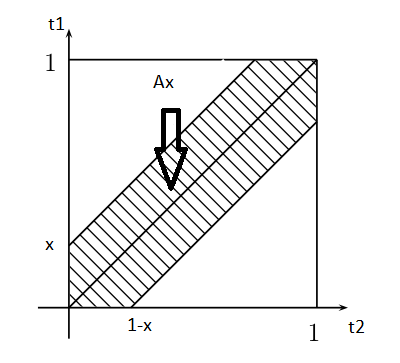
\includegraphics[width=0.5\linewidth]{img/vstr1.png}
      \caption{Задача о встрече}
    \end{figure}
	
	$\xi((\omega)=(t_1,t_2)) = |t_1 - t_2|$	 
	\begin{equation*}
		F_{\xi}(x) = \mathbb{P} \{ \xi < x \} = \mathbb{P} \{ \omega \in \Omega : |t_1 - t_2| < x \} = \mathbb{P}
			\begin{cases}
				\varnothing , x \leq 0 \\			
				A_x, x \in (0,1)\\ 
				\Omega, x > 1
			\end{cases}
	\end{equation*}
 
	\begin{equation*}
		=\mathbb{P}
			\begin{cases}
				0 , x \leq 0 \\			
				1-(1-x)^2, x \in (0,1)\\
				1, x > 1
			\end{cases}
	\end{equation*}
\end{zad}

\subsection{Основные дискретные распределения}
\subsubsection{Вырожденное}
\[ \xi \sim \left( \begin{array}{c}
	a \\ \hline
	1 \\
\end{array} \right) \]
$\xi \sim \boldsymbol{D}(a)$, $a \in \mathbb{R}$
\subsubsection{Биномиальное}
$\xi \sim \boldsymbol{Bi}(n,p)$, $n \in \mathbb{N}$, $p \in (0,1)$ -- параметр, $q=1-p$
\[ \xi \sim \left( \begin{array}{ccccc}
	0 & \multicolumn{1}{|c}{\cdots} & \multicolumn{1}{|c}{k} & \multicolumn{1}{|c}{\cdots} & \multicolumn{1}{|c}{n}\\ \hline
	q^{n} & \multicolumn{1}{|c}{\cdots} & \multicolumn{1}{|c}{\binom{n}{k}p^{k}q^{n-k}} & \multicolumn{1}{|c}{\cdots} & \multicolumn{1}{|c}{p^{n}}\\
\end{array} \right) \]
\subsubsection{Пуассоновское}
$\xi \sim \boldsymbol{\Pi}(\lambda)$, $\lambda > 0$ -- параметр,
\[ \xi \sim \left( \begin{array}{ccccc}
	0 & \multicolumn{1}{|c}{1} & \multicolumn{1}{|c}{\cdots} & \multicolumn{1}{|c}{k} & \multicolumn{1}{|c}{\cdots}\\ \hline
	e^{-\lambda} & \multicolumn{1}{|c}{\lambda e^{-\lambda}} & \multicolumn{1}{|c}{\cdots} & \multicolumn{1}{|c}{\frac{\lambda^{k}}{k!} e^{-\lambda}} & \multicolumn{1}{|c}{\cdots}\\
\end{array} \right) \]
\subsubsection{Геометрическое}
$\xi \sim \boldsymbol{G}(p)$, $p \in (0,1)$ -- параметр,
\[ \xi \sim \left( \begin{array}{ccccc}
	1 & \multicolumn{1}{|c}{2} & \multicolumn{1}{|c}{\cdots} & \multicolumn{1}{|c}{k} & \multicolumn{1}{|c}{\cdots}\\ \hline
	p & \multicolumn{1}{|c}{pq} & \multicolumn{1}{|c}{\cdots} & \multicolumn{1}{|c}{pq^{k-1}} & \multicolumn{1}{|c}{\cdots}\\
\end{array} \right) \]
\subsection{Основные абсолютно непрерывные распределения}
\subsubsection{Равномерное на отрезке}
$\xi \sim \boldsymbol{R}(a,b)$, $a$,$b \in \mathbb{R}$, $a < b$
\begin{equation*}
	\xi \sim f_{\xi}(x) = 
		\begin{cases}
			0 , x \notin [a,b] \\			
			\frac{1}{b-a}, x \in [a,b]
		\end{cases}
\end{equation*}
\begin{equation*}
	\xi \sim F_{\xi}(x) = 
		\begin{cases}
			0 , x \leq a \\			
			\frac{x-a}{b-a}, a \leq x \leq b \\
			1 , x \geq b
		\end{cases}
\end{equation*}
\begin{figure}[H]
      \centering
      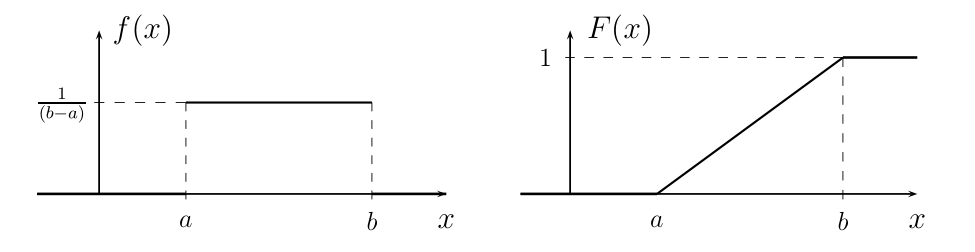
\includegraphics[width=0.8\linewidth]{img/ravnom1.png}
      \caption{Графики}
\end{figure}
\subsubsection{Нормальное}
$\xi \sim \mathcal{N}(a,\sigma^{2})$, $a \in \mathbb{R}$, $\sigma^{2} > 0$, $\sigma = +\sqrt{\sigma^{2}} > 0$

$\xi \sim f_{\xi}(x) = \frac{1}{\sqrt{2\pi\sigma^{2}}}e^{-\frac{(x-a)^{2}}{2\sigma^{2}}}$, $\forall x \in \mathbb{R}$
\begin{figure}[H]
      \centering
      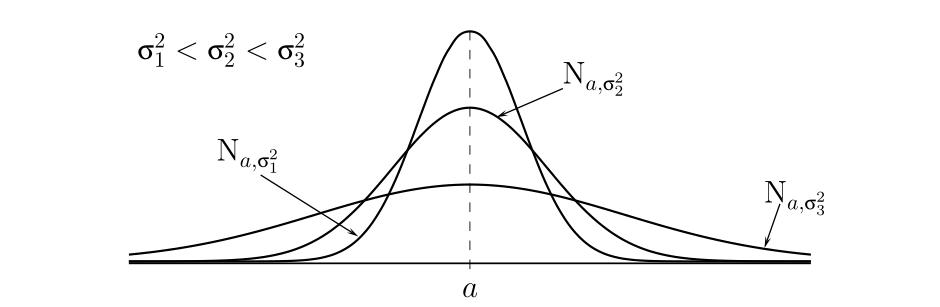
\includegraphics[width=0.8\linewidth]{img/plotnorm.png}
      \caption{Плотности нормальных распределений}
\end{figure}

$\xi \sim F_{\xi}(x) = \Phi \left( \frac{x-a}{\sigma} \right)$
\begin{figure}[H]
      \centering
      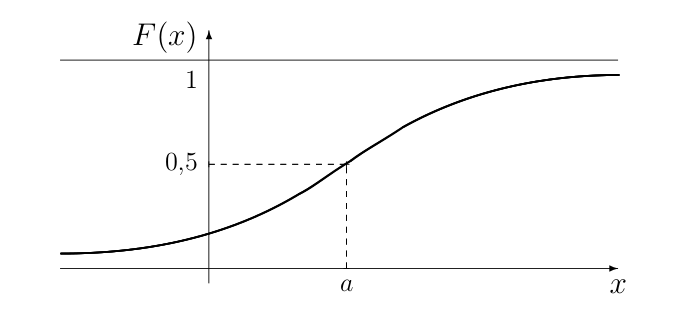
\includegraphics[width=0.8\linewidth]{img/frnorm.png}
      \caption{Функция распределения нормального распределения}
\end{figure}

Стандартное нормальное распределение:

$\xi \sim \mathcal{N}(0,1)$

$\xi \sim f_{\xi}(x) = \frac{1}{\sqrt{2\pi}} e^{-\frac{x^{2}}{2}}$

$\xi \sim F_{\xi}(x) = \Phi(x) = \int_{-\infty}^{x} \frac{1}{\sqrt{2\pi}} e^{-\frac{t^{2}}{2}} dt$ -- функция Лапласа

\subsubsection{Показательное}
$\xi \sim \boldsymbol{Exp}(\lambda)$, $\lambda > 0$, $\xi \sim \boldsymbol{Exp}(\lambda) = \boldsymbol{\Gamma}(1, \frac{1}{\lambda})$
\begin{equation*}
	\xi \sim f_{\xi}(x) = 
		\begin{cases}
			0 , x \leq 0 \\			
			\lambda e^{-\lambda x}, x > 0
		\end{cases}
\end{equation*}
\begin{equation*}
	\xi \sim F_{\xi}(x) = 
		\begin{cases}
			0 , x \leq 0 \\			
			1-e^{-\lambda x}, x > 0
		\end{cases}
\end{equation*}
\begin{figure}[H]
      \centering
      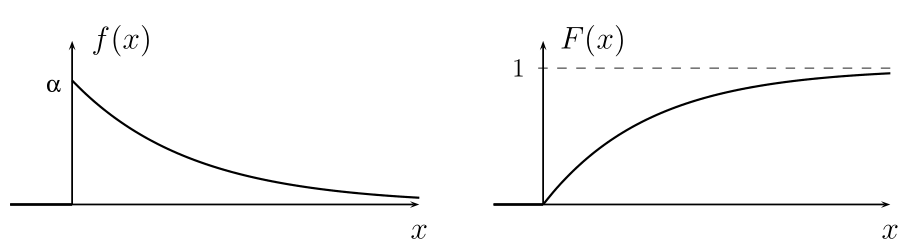
\includegraphics[width=0.8\linewidth]{img/expon.png}
      \caption{Плотность и функция распределения}
\end{figure}

\subsubsection{Гамма-распределение}
$\xi \sim \boldsymbol{\Gamma}(\alpha, \beta)$, $\alpha > 0$, $\beta > 0$
\begin{equation*}
	\xi \sim f_{\xi}(x) = 
		\begin{cases}
			0 , x \leq 0 \\			
			\frac{x^{\alpha - 1}}{\Gamma(\alpha) \beta^{\alpha}} e^{-\frac{x}{\beta}}, x > 0
		\end{cases}
\end{equation*}
$\Gamma(\alpha) = \int_{0}^{+\infty} x^{\alpha -1} e^{-x} dx$

$\xi \sim F_{\xi}(x) = \int_{-\infty}^x f_{\xi}(t)dt$ -- явно не вычисляется.
\subsubsection{Хи-квадрат-распределение}
$\xi \sim \boldsymbol{\chi}_{2}^{\alpha} := \boldsymbol{\Gamma}(\frac{\alpha}{2}, 2)$, $\alpha > 0$
\begin{figure}[H]
      \centering
      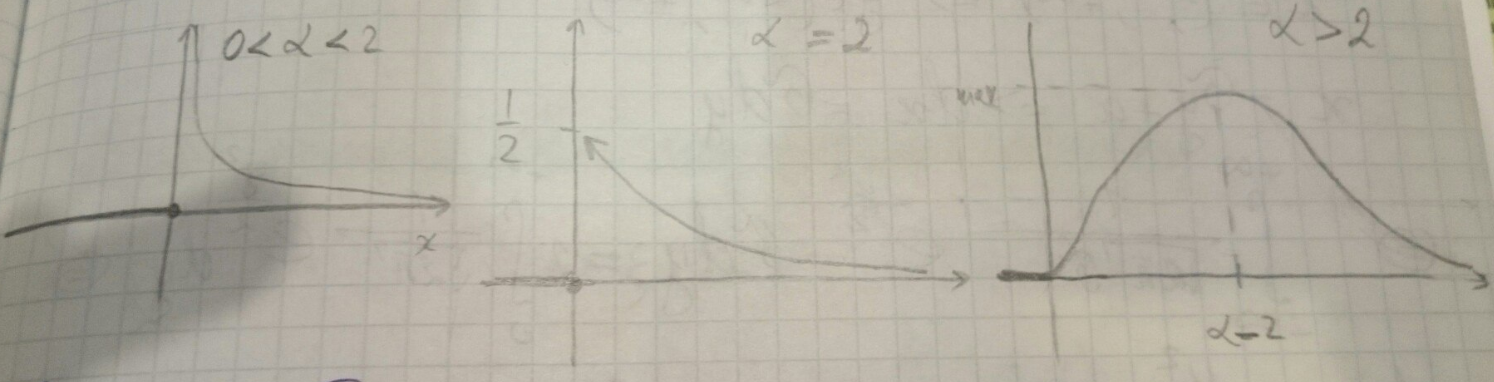
\includegraphics[width=0.8\linewidth]{img/chi.png}
      \caption{Плотность хи-квадрат-распределения}
\end{figure}